
\chapter[Estudo de Confiabilidade do Posicionador de Lente]{Estudo de Confiabilidade do Posicionador de Lente}

O projeto de um equipamento deve ser executado a fim de garantir que o mesmo permaneça operacional por um determinado intervalo de tempo, sem que falhas possam causar interrupções parciais ou totais, considerando como requisitos do projeto as condições ambientais associadas com sua operação e condições de uso específicas.

Uma maneira de definir a confiabilidade de um produto é a repetitividade que o sistemas possui em executar uma função, por um período de tempo, sob condições previamente definidas. A análise de confiabilidade deve definir os seguintes pontos:
\begin{itemize}
\item Principais modos de falha associados aos componentes do sistema;
\item Comportamento estatístico de falha associados a estes componentes;
\item Progressão de falha de um componente ao longo do sistema e as suas consequências sobre a operacionalidade do mesmo.
\end{itemize}

“A probabilidade de um sistema ou item desempenhar satisfatoriamente a função requerida, sob condições de operação estabelecidas, por um período de tempo pré-determinado”, \cite{lewis}.

As análises de confiabilidade aqui mostrada serão baseadas em dados probabilísticos, mas com aplicações de metodologias estatísticas adequadas, sendo assim, os resultados possuem aproximação aceitável. A figura \ref{confiabilidade} mostra os fatores que influenciam uma análise de confiabilidade.

\begin{figure}[htb]
		\centering
			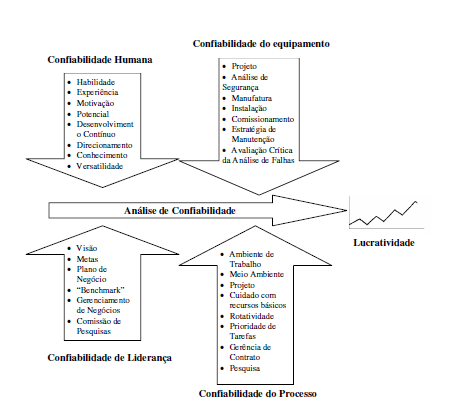
\includegraphics[scale=1.0]{figuras/confiabilidade.png}
		\caption{Análise de confiabilidade}
		\label{confiabilidade}
\end{figure}

A figura \ref{confiabilidade} mostra a importância de uma boa análise de confiabilidade no aumento dos lucros da organização. A confiabilidade foi implementada neste projeto desde o início, na fase de especificar e executar os testes nos componentes. Atualmente no desenvolvimento e, na fase final do desenvolvimento, realização de testes no produto.

Alguns pontos específicos são importantes:
\begin{itemize}
\item Desempenho específico é esperado;
\item Condições de uso devem ser especificadas;
\item Há um período de tempo de utilização;
\item A função do equipamento deve ser claramente definida, pois isso permite reconhecer as causas de falha;
\item Ambiente, ações de manutenção e operação;
\item O tempo de utilização;
\end{itemize}

A análise do comportamento da taxa de falha de um equipamento genérico por um período de tempo, pode ser representada pela curva de componentes elétricos e eletrônicos da figura \ref{banheira}, conhecida como Curva da Banheira \cite{castro}.

\begin{figure}[H]
		\centering
			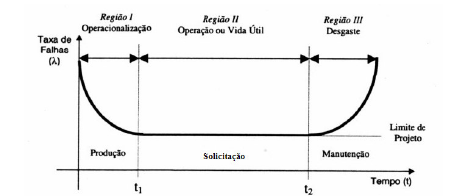
\includegraphics[scale=1.0]{figuras/banheira.png}
		\caption{Representação da Curva da Banheira \cite{castro}}
		\label{banheira}
\end{figure}

A região I do gráfico denomina se de região de falhas precoces. Estas falhas estão relacionadas a problemas associados ás matérias primas utilizadas ou aos processos de fabricação e montagem. A região II da curva representa o período de vida útil do produto, onde se apresenta a menor taxa de falha. Nesta região as falhas são aleatórias e originadas por solicitações maiores que o esperado no projeto, como por exemplo, vibrações, variação de tensão, impactos mecânicos, oscilação de temperatura e umidade. Quando esta taxa se torna crescente, inicia se a região III. A região III, ou região de desgaste identifica que o período de operação e os seus componentes começam a apresentar falhas associadas à danos cumulativos.


\textbf{Árvore Funcional}

A execução da análise do sistema deve ser sistematizada, baseando se em uma descrição das funções de cada um dos componentes, bem como a ligação entre eles, de forma a caracterizar a estrutura física deste em termos das relações funcionais entre seus componentes. A execução da árvore funcional mostrada na figura \ref{arvore} permite um registro claro da função de cada um dos componentes do sistema, subsidiando a execução da próxima etapa.

\begin{figure}[H]
		\centering
			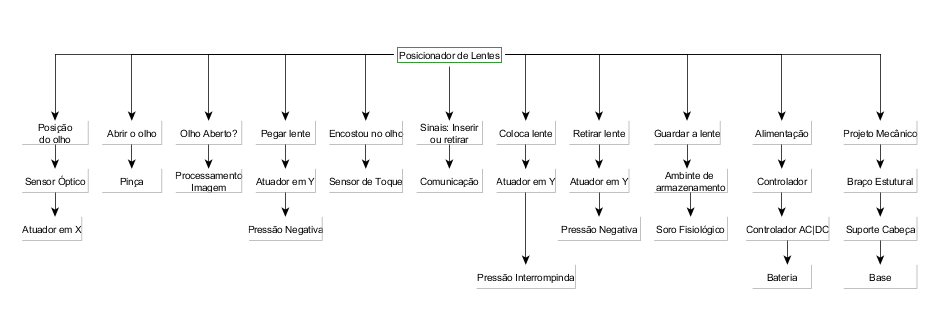
\includegraphics[scale=1.0, angle=90]{figuras/arvore.png}
		\caption{Arranjo Árvore Funcional de Posicionador de Lentes}
		\label{arvore}
\end{figure}


\textbf{FMEA}

A análise de modos de efeito de falha (FMEA, do inglês “Failure Models and Effects Analysis”), tem por objetivo verificar as consequências da falha de um componente sobre a operacionalidade do sistema.

A execução da análise do tipo FMEA se inicia com a definição de possíveis modos de falha dos componentes d um sistema. A cada modo de falha estão relacionadas possíveis causas, que se relacionam com fenômenos físicos que ocorrem durante a operação, fabricação ou montagem dos componentes.

Levantados os modos de falha, procede-se a uma avaliação de consequências da ocorrência de qualquer uma das falhas sobre o sistema. A proporção que a falha acarretará no sistema depende das características operacionais do sistema eletrônico total.

Como método, o FMEA tem diretrizes gerais as quais devem ser seguidos. Dessa forma é necessário responder as seguintes questões sobre o sistema:
\begin{itemize}
\item Como cada componente do sistema pode falhar?
\item Quais os efeitos que esta falha trará ao sistema?
\item Quão críticos serão esses efeitos?
\item Como detectar a falha?
\item Quais as medidas que podem evitar a falha?
\end{itemize}

A análise a partir do FMEA baseia se na execução de uma tabela, similar as figuras \ref{confisensores}, \ref{confiatuadores}, \ref{confipinca}, \ref{confiimagens}, \ref{confiarmazenamento} e \ref{confibraco} que representam o número mínimo de informações para execução de uma análise adequada. Na primeira coluna apresenta se a descrição da função do componente, indicando a sua relação com o sistema de estudo. Na segunda coluna descrevem se as possíveis falhas que podem ser apresentadas pelo componente e em qual modo de operação do sistema. Eventualmente, poderão ser listados todos os possíveis modos de falha do componente, pois, dependendo do tipo de sistema em análise, do ambiente em que este operará, ou outras causas, apenas alguns modos de falha se aplicam ao caso em estudo, devendo esta hipótese ser claramente especificada na análise. A seguir, nas figuras \ref{confisensores}, \ref{confiatuadores}, \ref{confipinca}, \ref{confiimagens}, \ref{confiarmazenamento} e \ref{confibraco}, são discutidas as ações recomendadas e a ocorrência e severidade que cada falha pode gerar no sistema.



\begin{figure}[H]
		\centering
			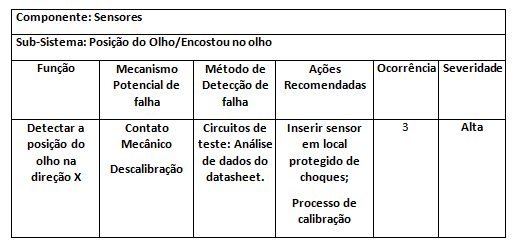
\includegraphics[scale=1.0]{figuras/confisensores.png}
		\caption{Informações para Elaboração da Análise de Modos de Efeito de Falhas SAE 1739- Adaptado para sensores \cite{sae}}
		\label{confisensores}
\end{figure}

\begin{figure}[H]
		\centering
			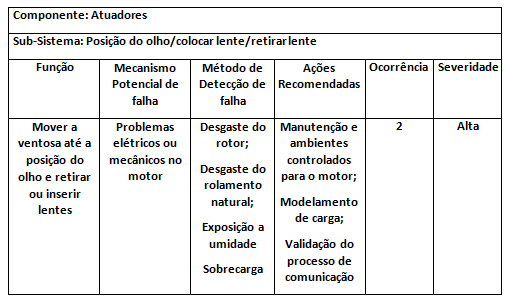
\includegraphics[scale=1.0]{figuras/confiatuadores.png}
		\caption{Informações para Elaboração da Análise de Modos de Efeito de Falhas SAE 1739- Adaptado para Atuadores \cite{sae}}
		\label{confiatuadores}
\end{figure}

\begin{figure}[H]
		\centering
			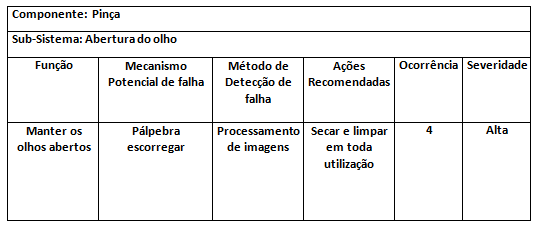
\includegraphics[scale=1.0]{figuras/confipinca.png}
		\caption{Informações para Elaboração da Análise de Modos de Efeito de Falhas SAE 1739- Adaptado para pinça \cite{sae}}
		\label{confipinca}
\end{figure}

\begin{figure}[H]
		\centering
			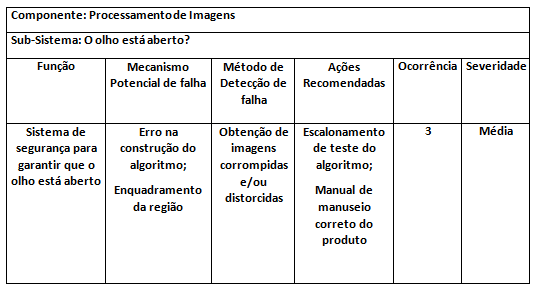
\includegraphics[scale=1.0]{figuras/confiimagens.png}
		\caption{Informações para Elaboração da Análise de Modos de Efeito de Falhas SAE 1739- Adaptado para Processamento de imagens \cite{sae}}
		\label{confiimagens}
\end{figure}

\begin{figure}[H]
		\centering
			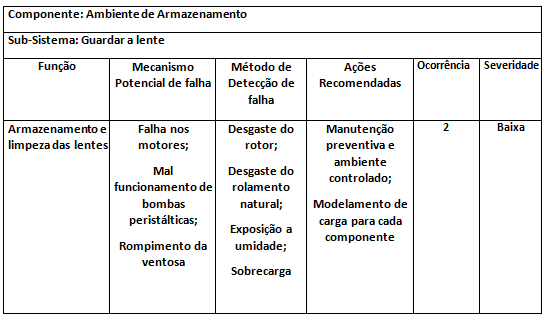
\includegraphics[scale=1.0]{figuras/confiarmazenamento.png}
		\caption{Informações para Elaboração da Análise de Modos de Efeito de Falhas SAE 1739- Adaptado para Ambiente de armazenamento \cite{sae}}
		\label{confiarmazenamento}
\end{figure}

\begin{figure}[H]
		\centering
			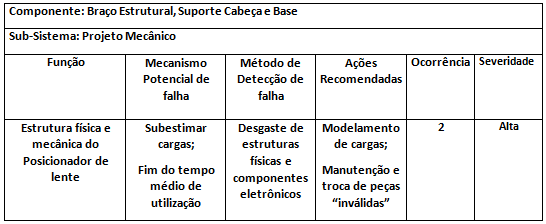
\includegraphics[scale=1.0]{figuras/confibraco.png}
		\caption{Informações para Elaboração da Análise de Modos de Efeito de Falhas SAE 1739- Adaptado para Braço Estrutural, Suporte Cabeça e Base \cite{sae}}
		\label{confibraco}
\end{figure}

A classificação da severidade de um modo de falha, que tem como objetivo fornecer uma idéia qualitativa do efeito do modo de falha do componente sobre o sistema como um todo. A figura \ref{severidade} mostra como é feita essa classificação. As normas indicam os valores de Ocorrência em escalas de 1 a 10. Quanto maior esse índice, maior é a chance de ocorrer um dado modo de falha.

\begin{figure}[H]
		\centering
			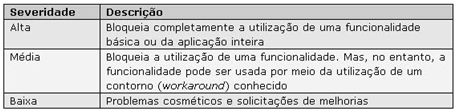
\includegraphics[scale=1.0]{figuras/severidade.png}
		\caption{Classificação de Severidade conforme a \citeonline{sae}}
		\label{severidade}
\end{figure}